% !TEX root = ../SYSprojektrapport.tex
% SKAL STÅ I TOPPEN AF ALLE FILER FOR AT MASTER-filen KOMPILERES 

\section{Case 3: Husstandsbatteriers evne til at kompensere for tab af produktion}
I dette afsnit præsenteres resultater for simuleringen af case 3 iht. beskrivelsen i afsnit \ref{SimCase1}. I alle fire tilstande er spændingsændringen ved \textit{Town5 busbar} (rød linje) og \textit{Transmission central 60kV busbar} (Grøn linje) samt frekvensændringen på \textit{Transmission central 60kV busbar} (Grøn linje) præsenteret på hhv. spændingsgraf og frekvensgraf. Derudover er der lavet opsamling over spænding samt effektoverførelse andre relevante steder i systemet i tabel \ref{fig:C3Overview}. \\ \\

\newpage
\textbf{Tilstand 1: Alle batterierne er frakoblet.}
\begin{figure}[H]
	\centering
	\begin{minipage}[b]{0.48\textwidth}
		\centering
		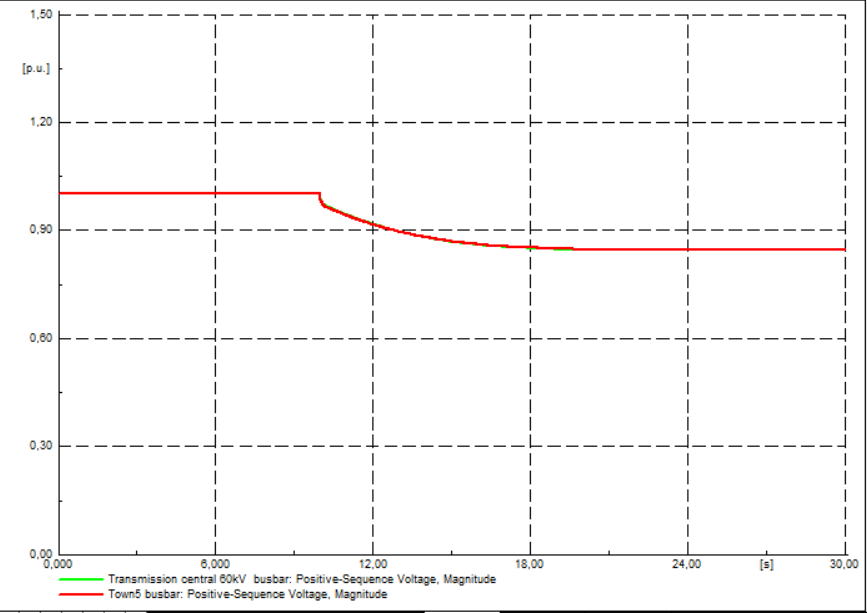
\includegraphics[width=1.00\textwidth]{figurer/LargeDisturbance/Voltage1} % Venstre billede
	\end{minipage}
	\hfill
	\begin{minipage}[b]{0.48\textwidth}
		\centering
		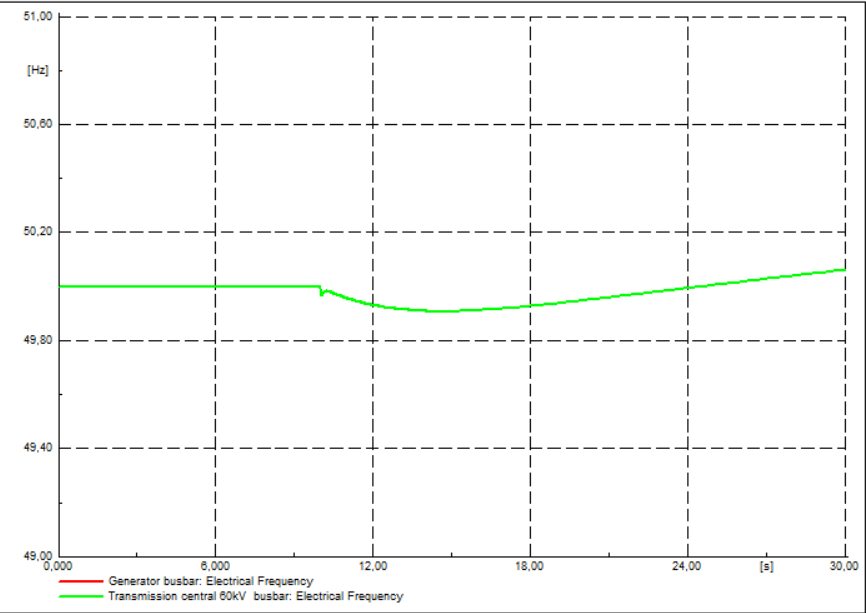
\includegraphics[width=1.00\textwidth]{figurer/LargeDisturbance/Freq1} % Højre billede
	\end{minipage}
	\\ % Figurtekster og labels
	\begin{minipage}[t]{0.48\textwidth}
		\caption{Case 3, Tilstand 1, Spændingsgraf} % Venstre figurtekst og label
		\label{fig:C3T1V}
	\end{minipage}
	\hfill
	\begin{minipage}[t]{0.48\textwidth}
		\caption{Case 3, Tilstand 1, Frekvensgraf} % Højre figurtekst og label
		\label{fig:C3T1F}
	\end{minipage}
\end{figure}

\textbf{Tilstand 2: Alle batterier leverer 0,5MW med pf 0,95 lagging.}
\begin{figure}[H]
	\centering
	\begin{minipage}[b]{0.48\textwidth}
		\centering
		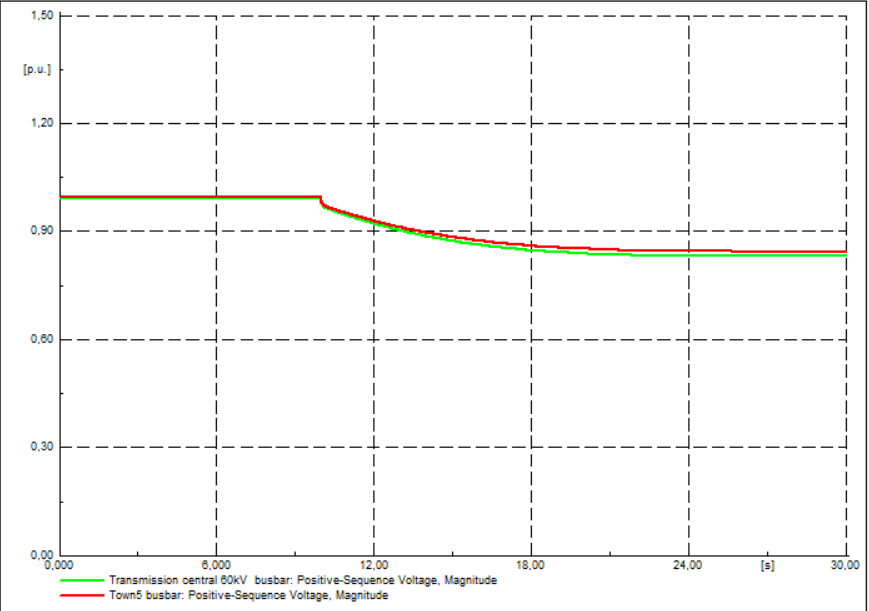
\includegraphics[width=1.00\textwidth]{figurer/LargeDisturbance/Voltage2} % Venstre billede
	\end{minipage}
	\hfill
	\begin{minipage}[b]{0.48\textwidth}
		\centering
		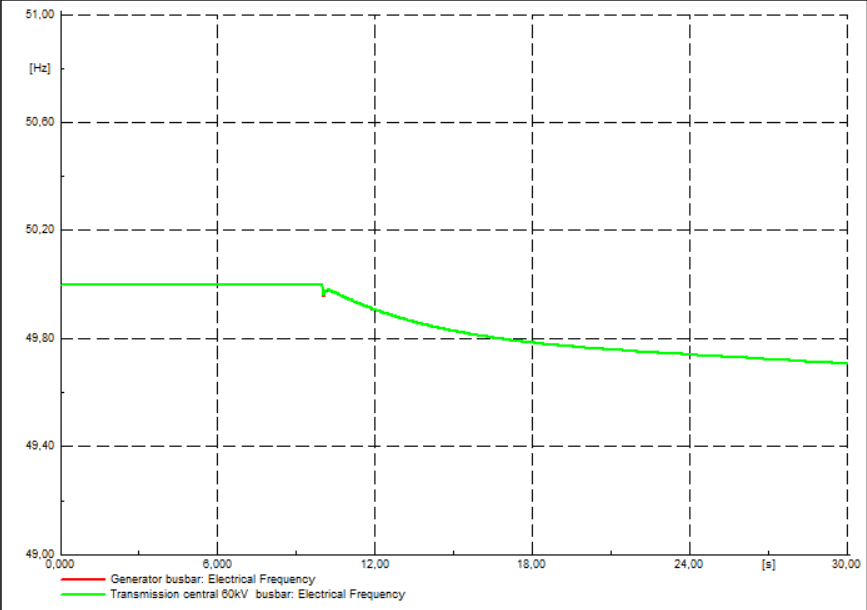
\includegraphics[width=1.00\textwidth]{figurer/LargeDisturbance/Freq2} % Højre billede
	\end{minipage}
	\\ % Figurtekster og labels
	\begin{minipage}[t]{0.48\textwidth}
		\caption{Case 3, Tilstand 2, Spændingsgraf} % Venstre figurtekst og label
		\label{fig:C3T2V}
	\end{minipage}
	\hfill
	\begin{minipage}[t]{0.48\textwidth}
		\caption{Case 3, Tilstand 2, Frekvensgraf} % Højre figurtekst og label
		\label{fig:C3T2F}
	\end{minipage}
\end{figure}

\textbf{Tilstand 3: Alle batterier leverer 1MW med pf 0,95 lagging.}
\begin{figure}[H]
	\centering
	\begin{minipage}[b]{0.48\textwidth}
		\centering
		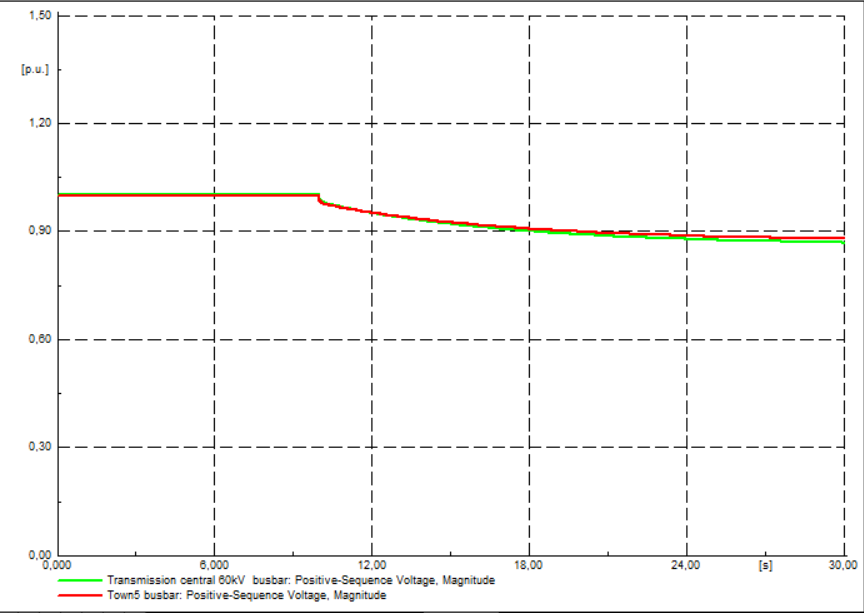
\includegraphics[width=1.00\textwidth]{figurer/LargeDisturbance/Voltage3} % Venstre billede
	\end{minipage}
	\hfill
	\begin{minipage}[b]{0.48\textwidth}
		\centering
		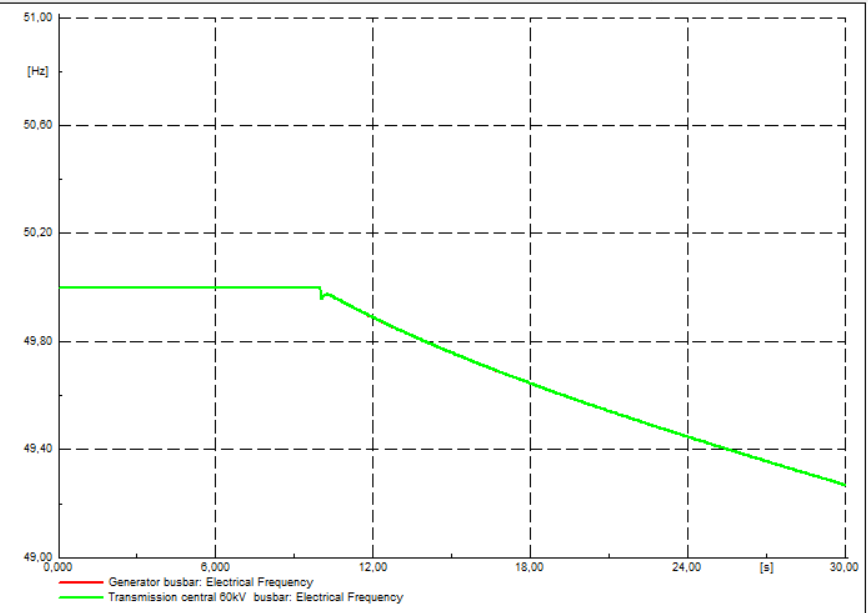
\includegraphics[width=1.00\textwidth]{figurer/LargeDisturbance/Freq3} % Højre billede
	\end{minipage}
	\\ % Figurtekster og labels
	\begin{minipage}[t]{0.48\textwidth}
		\caption{Case 3, Tilstand 3, Spændingsgraf} % Venstre figurtekst og label
		\label{fig:C3T3V}
	\end{minipage}
	\hfill
	\begin{minipage}[t]{0.48\textwidth}
		\caption{Case 3, Tilstand 3, Frekvensgraf} % Højre figurtekst og label
		\label{fig:C3T3F}
	\end{minipage}
\end{figure}

\textbf{Tilstand 4: Alle batterier leverer 1,35MW (Byerne kan betegnes som selvforsynende) med pf 0,95 lagging.}
\begin{figure}[H]
	\centering
	\begin{minipage}[b]{0.48\textwidth}
		\centering
		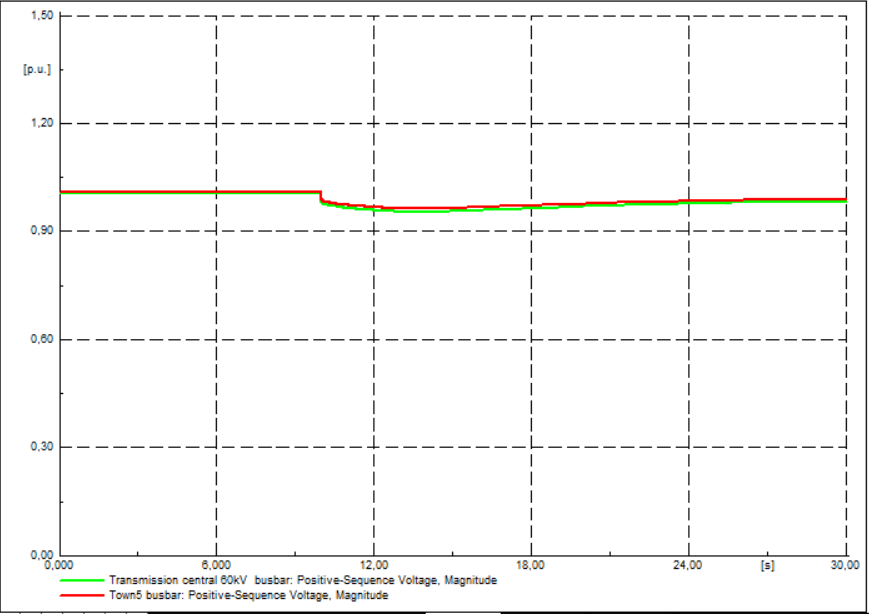
\includegraphics[width=1.00\textwidth]{figurer/LargeDisturbance/Voltage4} % Venstre billede
	\end{minipage}
	\hfill
	\begin{minipage}[b]{0.48\textwidth}
		\centering
		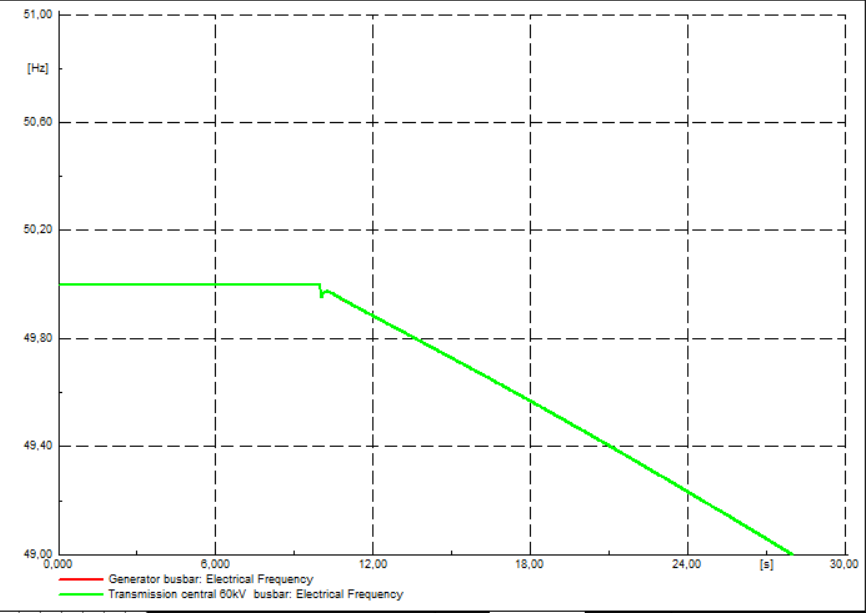
\includegraphics[width=1.00\textwidth]{figurer/LargeDisturbance/Freq4} % Højre billede
	\end{minipage}
	\\ % Figurtekster og labels
	\begin{minipage}[t]{0.48\textwidth}
		\caption{Case 3, Tilstand 4, Spændingsgraf} % Venstre figurtekst og label
		\label{fig:C3T4V}
	\end{minipage}
	\hfill
	\begin{minipage}[t]{0.48\textwidth}
		\caption{Case 3, Tilstand 4, Frekvensgraf} % Højre figurtekst og label
		\label{fig:C3T4F}
	\end{minipage}
\end{figure}

\textbf{Tilstandsoverblik}
\begin{figure}[H] % (alternativt [H])
	\centering
	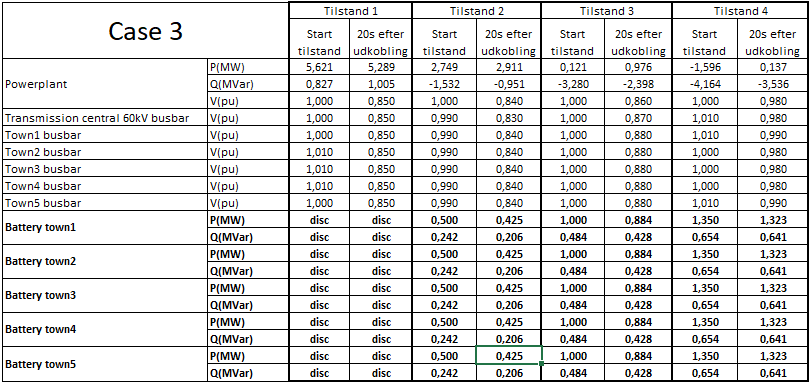
\includegraphics[width=1\textwidth]{figurer/LargeDisturbance/Overview}
	\caption{Overblik for spænding og effektoverførelse i nettet}
	\label{fig:C3Overview}
\end{figure}

Der observeres at når produktionen fra vindmølleparken udkobles vil der opleves et spændingsfald på både \textit{Town5 busbar} - \textit{Town5 busbar} er repræsentativ for alle byer - og \textit{Transmission central 60kV busbar}. Det ses at spændingsfaldet i per unit er af samme størrelsesorden for både \textit{Town5 busbar} og \textit{Transmission central 60kV busbar}. På spændingsgraferne ses det at en stor andel af effektbidrag fra batteri vil resultere i et mindre spændingsfald ved udkobling. Dette skyldes det lavere effektbidrag fra synkron generatoren og derved mindre strøm i transmissions- og distrbutionskabler. I tilstand 4, hvor byerne er selvforsynende - jf. effektbidraget 20s efter udkobling fra Powerpant i tabel \ref{fig:C3Overview} -  ses kun et lille spændingsfald efterfulgt af en spændingsstigning. Spændingen vil stabilisere sig selv efter udkoblingen pga. at produktion og belastning ligger samme sted og der derfor er en meget lille kildeimpedans mellem produktion og belastning.

I forhold til frekvensen observeres det at når andelen af effektbidrag fra batterier øges ses der større fald i frekvensen. Dette tyder på at angående frekvensstabilitet i case 2 er en øget andel forsyning fra husstandsbatterier en ulempe. Grunden til dette er at systemet mister inerti, når synkron generatoren næsten ikke leverer effekt. Synkron generatoren er i dette system kritisk i forhold til inertien, da den er den eneste enhed, der bidrager med inerti. Der observeres i tilstand 1 at frekvensen falder efterfulgt af en frekvensstigning. Dette sker på baggrund af den regulering der er i synkron generatoren, da den vil forsøge at kompensere for tabet af vindmølleparken, imens spændingsfaldet vil resultere en mindre belastning. På et tidspunkt vil produktionen derfor bliver større end forbruget og resultere i en frekvensstigning.